\chapter{Implementación del sistema de reconocimiento de gestos propuesto}\label{capit:cap4}
\vspace{-2.0325ex}%
\noindent
\rule{\textwidth}{0.5pt}
\vspace{-5.5ex}% 
\newcommand{\pushline}{\Indp}% Indent puede ir o no :p

En este cap\'itulo se describen los detalles de implementación de cada etapa del sistema.   

\section{Adquisición de los datos}\label{sec:AdquisicionDatos}

Como se vio en el Capítulo \ref{capit:cap3} Sección \ref{sec:KinectSensor} los datos provienen de los sensores de profundidad de dos dispositivos Kinect, estos se encuentran ubicados uno frente al usuario (Kinect frontal), y otro al lado  izquierdo (Kinect lateral), con una distancia de $74$ y $79$ $cm.$ respectivamente; y entre ellos de $46$ $cm.$ como se muestra en la Figura \ref{fig:SetupSystem}.
\begin{figure}[!h]
\begin{center}
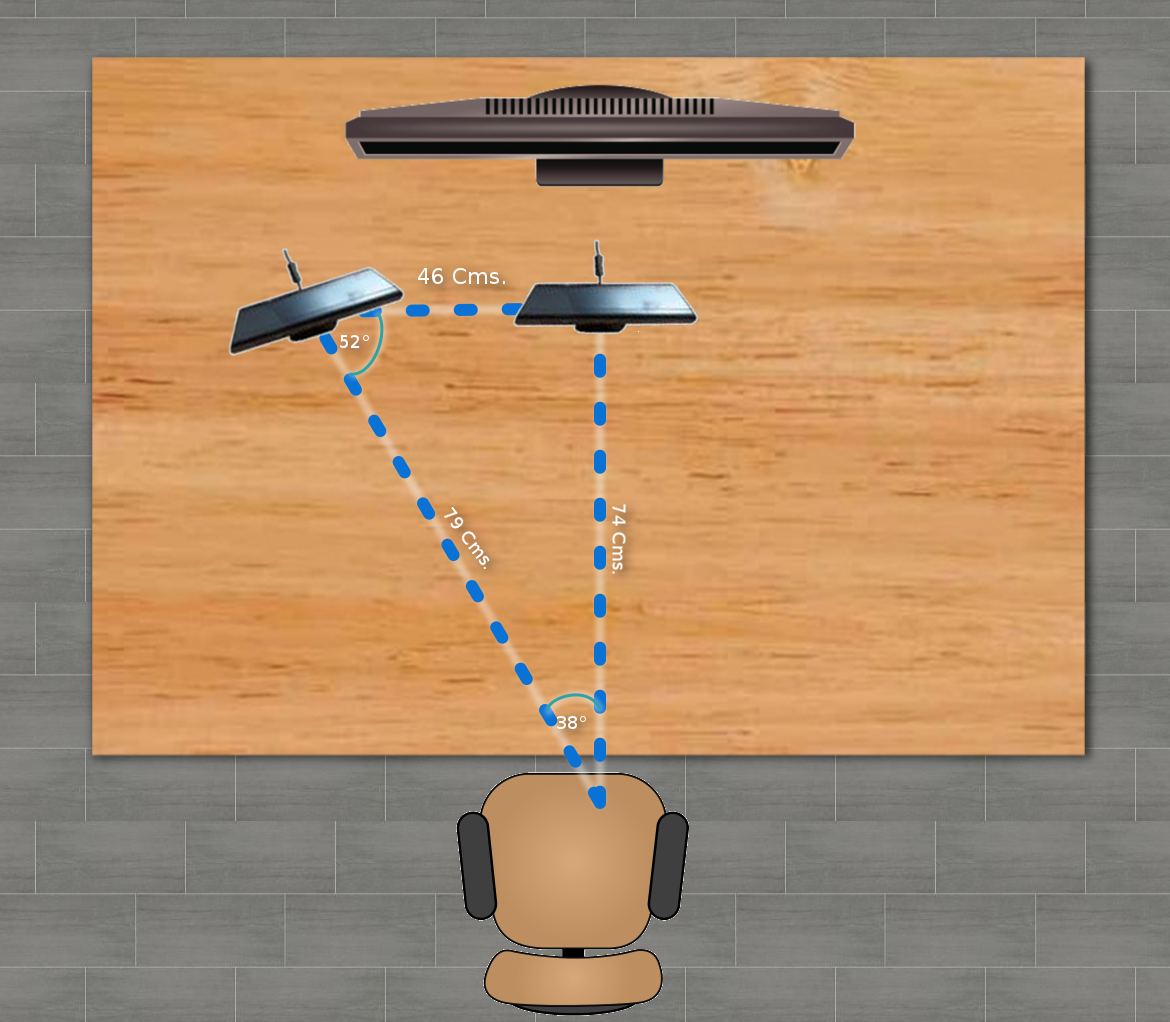
\includegraphics[scale=.2]{./Figures/system.png}
\end{center}
\caption{Configuración del sistema de reconocimiento de gestos}
\label{fig:SetupSystem}
\end{figure}  

Una vez que el flujo de datos de los sensores de profundidad es capturado este es representado como una imagen en escala de grises de $8$ bits de $640$ p\'ixeles de ancho por $480$ p\'ixeles de largo. En las imágenes se puede apreciar detalles pequeños, es decir cambios en la profundidad de hasta $1$  $mm.$ esto debido a que la escala de grises inicia cada $26$  $cm$. 
En la siguiente imagen se puede apreciar un ejemplo de las imágenes de profundidad, Figura \ref{fig:ImagenCapturada}

\begin{figure}[h!]
\begin{center}
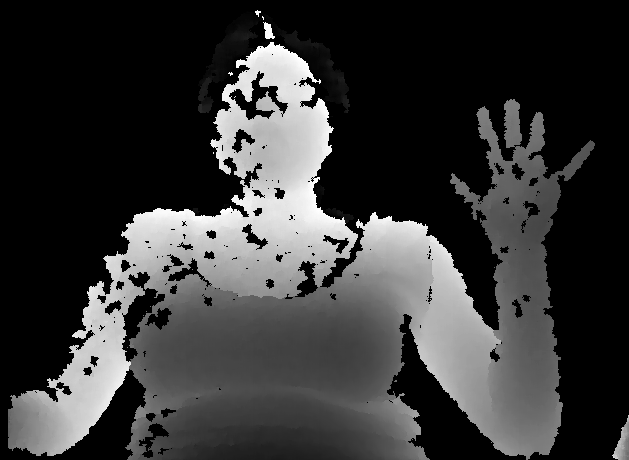
\includegraphics[scale=.35]{./Figures/166.png}
\end{center}
\caption{Representación de los datos capturados por los Kinect}
\label{fig:ImagenCapturada}
\end{figure}  

Por la naturaleza del Kinect, las imágenes obtenidas de ambos sensores contiene ruido, como el se muestra en la Figura \ref{fig:ImagenCapturadaNoNoise}; el ruido es reducido usando un filtro de mediana, este es aplicado en toda la imagen usando una ventada de tamaño $13$. La imagen resultante $S(x,y)$ es como la que se muestra en la Figura \ref{fig:ImagenCapturadaNoNoise}.\\ 
\begin{figure}[h!]
\begin{center}
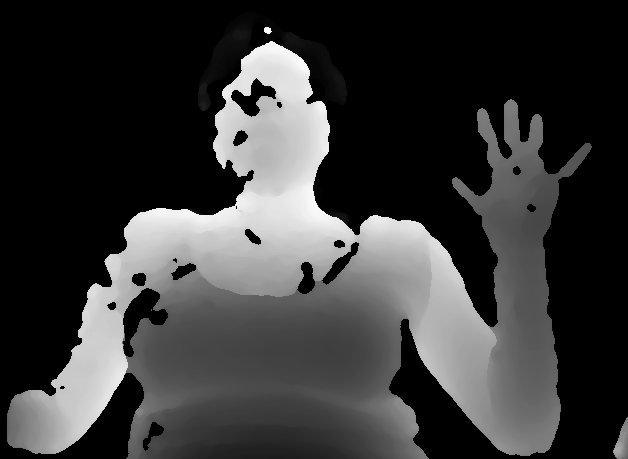
\includegraphics[scale=.35]{./Figures/166_W13.png}
\end{center}
\caption{Representación de los datos capturados por los Kinect}
\label{fig:ImagenCapturadaNoNoise}
\end{figure}  
Se aprecia en la imagen siguiente  que gran parte del ruido es reducido obteniendo una mejora en la imagen, desafortunadamente todavía existe ruido en la imagen, este puede ser eliminado casi en su mayoría  si el tamaño de la ventana aumenta pero se pierde información importante de la imagen, de manera que se decidió optar por el tamaño de ventana, antes mencionado. En la imagen también se aprecia el fondo negro, esto es debido a que se discrimino el fondo lo que estuviera a un distancia de más de $2$ $m.$ del sensor. 



\section{Detección}\label{sec:DeteccionSystem} 

En este trabajo se utiliza el algoritmo de detección de objetos desarrollado por Viola y Jones (2001), como se mostró en el Cap\'itulo \ref{capit:cap3} Sección \ref{subsec:ViolaJones}, el algoritmo clasifica las imágenes basándose en el valor de características, el clasificador es construido usando el algoritmo de AdaBoost en forma de cascada. 


La selección de las características se llev\'o acabo por medio de una versión modificada del algoritmo AdaBoost; la implementaci\'on se realiz\'o utilizando el software OpenCV Haar training classifier \footnote{{https://github.com/mrnugget/opencv-haar-classifier-training}}. Se entren\'o con $1000$ imágenes positivas (imágenes de profundidad de la mano), y $2000$ negativas, (imágenes de fondo de distintos escenarios). Las imágenes positivas fueron generadas de $300$ imágenes de poses; $3$ poses distintas, $100$ de cada pose, usando el software Create Samples \footnote{\url{http://note.sonots.com/SciSoftware/haartraining.html}}. Todas las imágenes usadas fueron tomadas de nuestra base de  datos \footnote{\label{myrepo} https://github.com/americamm}.

Nuestra base de datos contiene gran cantidad de imágenes de profundidad. Imágenes de fondo y de poses de la mano, estas fueron tomadas a una distancia de entre $60$ y $200$ $cm$. Las imágenes de profundidad de la mano fueron tomadas de $6$ personas distintas con tres distintas poses: palma con los dedos separados, como en la Figura \ref{fig:ImagenesPoses:2}, palma con dedos juntos, ver Figura \ref{fig:ImagenesPoses:3} y finalmente el pu\~no, ver Figura \ref{fig:ImagenesPoses:1}, como se muestran en la Figura \ref{fig:ImagenesPoses}. Las imágenes de fondo fueron tomadas de distintos escenarios como se muestra en la Figura \ref{fig:ImagenFondo}. El programa de captura de las imágenes puede ser encontrado en Github \ref{myrepo}.  

\begin{figure}[h!]
\begin{center}
\subfigure[Palma de la mano con los dedos separados.]{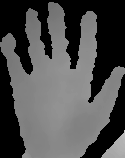
\includegraphics[scale=1]{./Figures/TrainingImage2.png}\label{fig:ImagenesPoses:2}}      \quad
\subfigure[Puño.]{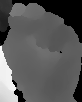
\includegraphics[scale=1.55]{./Figures/TrainingImage1.png}\label{fig:ImagenesPoses:1}}   \quad
\subfigure[Palma de la mano con los dedos juntos.]{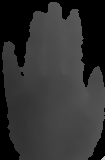
\includegraphics[scale=.99]{./Figures/TrainingImage3.png}\label{fig:ImagenesPoses:3}}
\end{center}
\caption{Ejemplo de imágenes de poses de nuestra base de datos.}
\label{fig:ImagenesPoses}
\end{figure}  

\begin{figure}[h!]
\begin{center}
\subfigure[Ejemplo de imagen de fondo, donde se encuentra una silla y escritorio.]{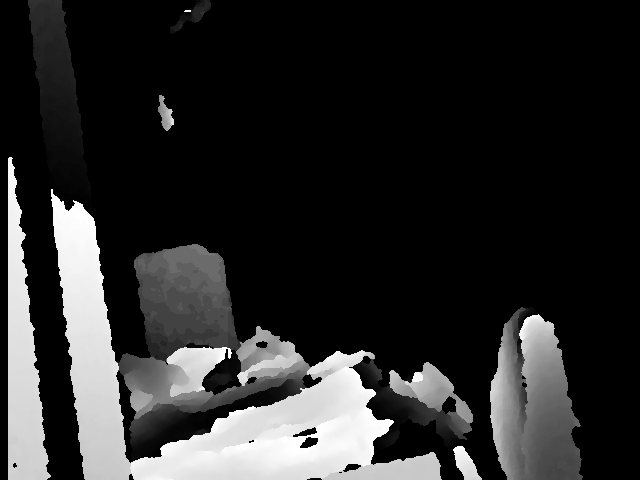
\includegraphics[scale=.3]{./Figures/Fondo5262.png}}\quad 
\subfigure[Ejemplo de imagen de fondo, donde se aprecian objetos en un escritorio.]{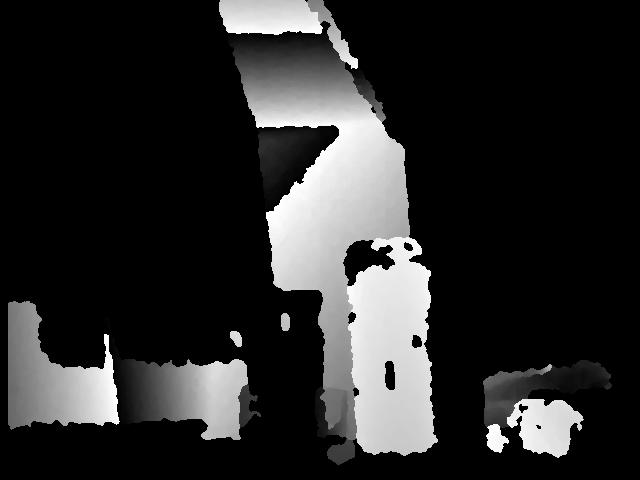
\includegraphics[scale=.3]{./Figures/Fondo11313.png}}\quad 
\end{center}
\caption{Imágenes del fondo de nuestra base de datos.}
\label{fig:ImagenFondo}
\end{figure}  

Los parámetros utilizados para la obtención del clasificador final fueron: el porcentaje de precision de detección de [$95%$] y la tasa de falsos positivos aceptados de [$5%$]. El resultado final del entrenamiento fue en clasificador AdoBoost en forma de cascada, que consta de 19 etapas. El clasificador resultante se encuentra en Github \ref{myrepo}, en formato XML.  

Con el clasificador obtenido, se localiza la mano en cada cuadro proveniente de los dispositivos  Kinect, una ventana  inicial de tamaño $60 \times 60$ pixeles se desliza por la imagen. Para eliminar falsos positivos que pudieran ocurrir en la detección de la mano se utiliza un algoritmo equivalente al de \cite{Mei2015}, este se muestra en el apéndice \ref{chap:apendA}.\\ 
Una vez que la mano se localiza la región de interés $ROI(x,y)$ es seleccionada alrededor de la mano, como se observa en la Figura \ref{fig:Roi}.

\begin{figure}[h!]
\begin{center}
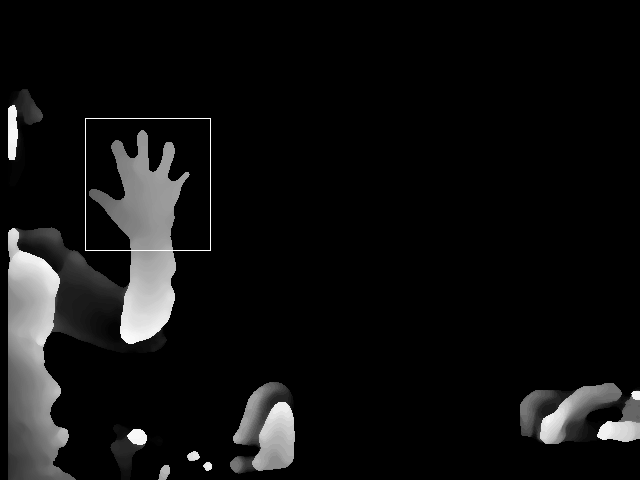
\includegraphics[scale=.35]{./Figures/DS_252.png}
\end{center}
\caption{Localización y selección de la mano, en la imagen de entrada del Kinect 2.}
\label{fig:Roi}
\end{figure}  

Ya que se tiene localizada el área donde se encuentra la mano, el siguiente paso es segmentar la mano del ROI. La segmentación se realiza binarizando el área del ROI, solo se toma esta área, para que el proceso sea más rápido. La binarizaci\'on se lleva acabo usando el algoritmo de Otsu, el resultado se muestra en la Figura \ref{fig:BinarizationRoi}. 
  
\begin{figure}[h!]
\begin{center}
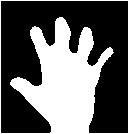
\includegraphics[scale=1]{./Figures/250B_Otsu.png}
\end{center}
\caption{Binarización de ROI y aplicación de las operaciones morfológicas a la mano localizada en la Figura anterior.}
\label{fig:BinarizationRoi}
\end{figure} 

%En la imagen [agregar imagen feita binarizada], se observa que el resultado de la bianrizacion no es el esperado. 
Para mejorar la binarizaci\'on, el ruido existe en la imagen es eliminado aplicando dos operaciones morfológicas, apertura y cierre, en respectivo ese orden. Las operaciones anteriores utilizan un elemento estructural rectangular. Para la operación de apertura el tamaño del elemento es de $3 \, x \, 9$ pixeles. Para el cierre se aplic\'o con un tamaño  $3\, x \, 11$ pixeles.

%\begin{figure}[h!]
%\begin{center} 
%\subfigure[]{
\includegraphics[scale=0.4]{./Figures/pusheen.png}\label{fig:HandNoNoises:1}}   \qquad
%\subfigure[]{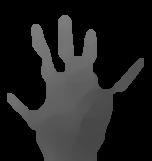
\includegraphics[scale=1.1]{./Figures/65_C.png}\label{fig:HandNoNoises:2}}  
%\end{center}
%\caption{La imágenes muestran el resultado de aplicar las operaciones morfológicas de apertura y cierre.}
%\label{fig:HandNoNoises}
%\end{figure}  


\section{Extracción de características}\label{sec:ExtraccionCaracteristicasSystem}

Como se vio en el Capítulo \ref{capit:cap3} Sección \ref{sec:Convexhull} las características de la mano son extraídas utilizando los algoritmos de envolvente convexa y  defectos de convexidad.

%\begin{figure}[!h]
%\begin{center}
%
\includegraphics[scale=.5]{./Figures/pusheen.png}
%\end{center}
%\caption{En esta dibujado la envolvente convexa, los puntos dibujados son los defectos de convexidad, en azul se encuentran los puntos de profundidad y en rojo los puntos de inicio.}
%\label{fig:Convex&Defects}
%\end{figure}

Una vez aplicados estos dos algoritmos se calcula: el número de dedos levantados, la posición de la punta de los dedos, la posición de la raíz de los dedos, el centro de la palma de mano, los ángulos que existe del centro de la mano a la punta de los dedos, los ángulos que existen del centro a la raíz de los dedos, la distancia que existe del centro de los dedos a la raíz de los dedos. En la Figura \ref{fig:FeaturesOfHand} se muestran algunas de estas características. Para la implementación de la extracción de las características, se tomo parte del código proveniente de un pagina de internet \footnote{http://blogs.ugidotnet.org/WetBlog/archive/2010/09/03/hand-gesture-recognition-powered-by-emgucv.aspx}. 

\begin{figure}[h!]
\begin{center} 
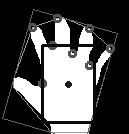
\includegraphics[scale=1]{./Figures/250_Dedos.png}
\end{center}
\caption{La imagen muestra algunas características de la mano. El contorno rojo representa la envolvente convexa, el rectángulo verde es el rectángulo que rodea a la mano, el rectángulo gris representa el área de la palma de la mano, los círculos en color amarillo la punta de los dedos, en color azul se encuentras los puntos de profundidad encontrados en medio de los dedos, en rosa el centro de la palma de la mano.}
\label{fig:FeaturesOfHand}
\end{figure}

Las características calculadas se guardan en un vector de características de dimensión $32$. El valor de la dimension del vector esta dada por la unión del conjunto de características obtenidas por cada imagen de la mano. En cada vector las características provenientes del Kinect 1 son almacenadas primero seguidas de las del Kinect 2.



%:::::::::::::::::::::::::::::::::::::::::::::::::::::::::::::::::::::::::::::::::::::::::::::::::::::::::::::::::::


\section{Reconocimiento}\label{sec:ReconocimientoSystem}

En este trabajo se reconocen gestos estáticos y dinámicos utilizando el método de maquinas de soporte vectorial.  

Como se vio en el Capitulo \ref{capit:cap3} Sección \ref{sec:SVM} SVM es un algoritmo de aprendizaje de máquina supervisado, por lo que es necesario tener imágenes de los gestos a reconocer. Con el conjunto de imágenes el clasificador es entrenado y el modelo de clasificación puede ser calculado. 

La implementación de SVM se lleva acabo usando LibSVMSharp \footnote{\url{https://github.com/ccerhan/LibSVMsharp}} un wrapper de la librería LibSVM \citep{Chang2011}.


\subsection{Reconocimiento de gestos estáticos}\label{RecognitionEstatic}

El sistema reconoce dos gestos estáticos: el puño y la palma de la mano con los dedos separados. El reconocimiento del gesto se lleva analizando un solo cuadro o imagen.  

El modelo que reconoce los gestos fue creado mediante SVM. Para el entrenamiento se tomaron $200$ imágenes de las dos distintas pose como las que se muestran en la Figura \ref{fig:SVMTrainingStatic}. Se utilizo un kernel exponencial y validación cruzada con 5 pliegues.   

\begin{figure}[h!]
\begin{center}
\subfigure[Palma de la mano con los dedos separados.]{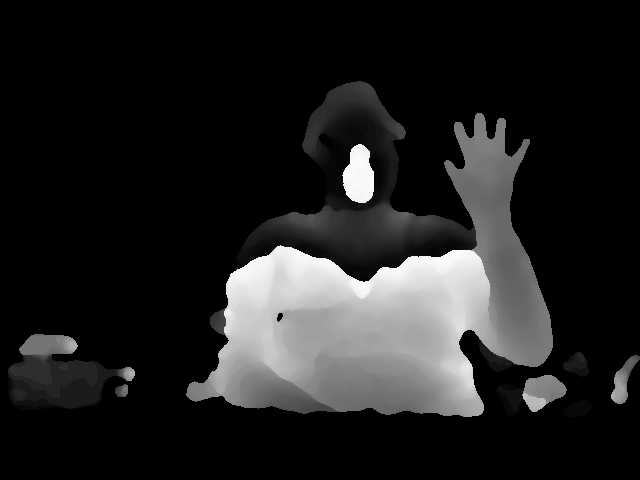
\includegraphics[scale=.3]{./Figures/G1.png}\label{fig:SVMTrainingStatic:1}}      \quad
\subfigure[Puño.]{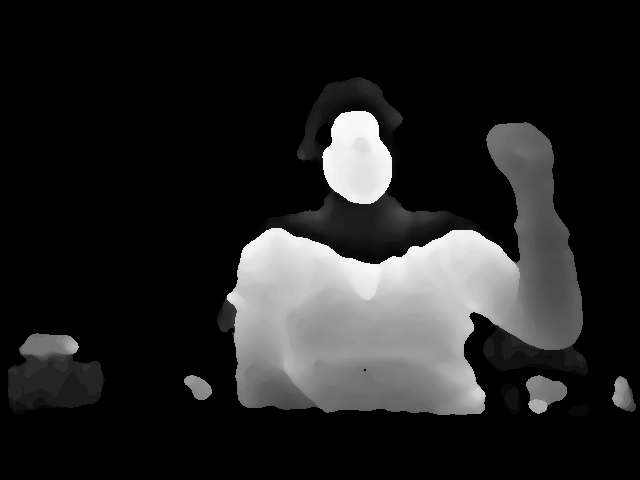
\includegraphics[scale=.3]{./Figures/G2.png}\label{fig:SVMTrainingStatic:2}}
\end{center}
\caption{Ejemplo de imágenes de poses de nuestra base de datos.}
\label{fig:SVMTrainingStatic}
\end{figure}


\subsection{Reconocimiento de gestos dinámicos}\label{RecognitionDynamic}


En este trabajo se toma un gesto dinámico como una secuencia de $30$ cuadros consecutivos en los cuales se realiza la misma pose en cada cuadro, solo que la pose cambian de posición, es decir se encuentra en movimiento. De manera que el sistema reconoce el gesto dinámico identificando y siguiendo cada pose en cada cuadro. La trayectoria del gesto es obtenida tomando en cuenta la posición del centro de la mano el cual es calculado en cada cuadro. 
 
El sistema reconoce dos gestos dinámicos, los cuales son los gestos estáticos en movimiento. La Figura \ref{fig:G3} muestra la secuencia del gesto dinámico de la palma de la mano. La Figura \ref{fig:G4} muestra a secuencia del gesto dinámico del mano en forma de pu\~no.  
\begin{figure}[h!]
\begin{center}
\subfigure[Cuadro inicial]{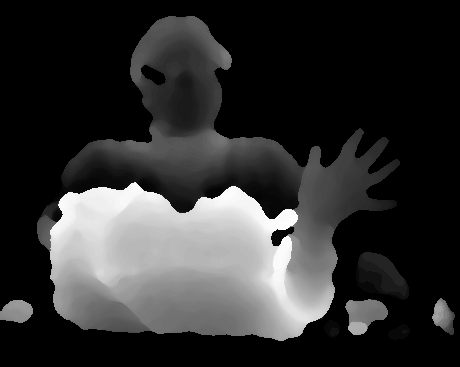
\includegraphics[scale=.25]{./Figures/G3_1.png}\label{fig:G3:1}}
\subfigure[Cuadro número 15 ]{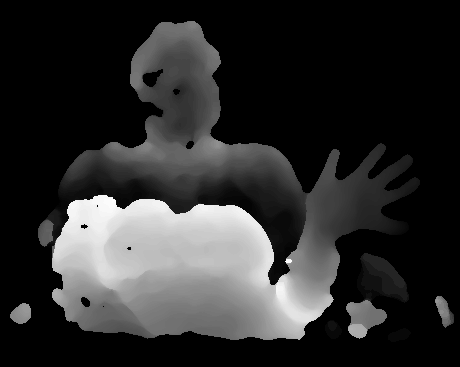
\includegraphics[scale=.25]{./Figures/G3_15.png}\label{fig:G3:2}}
\subfigure[Cuadro número 30 ]{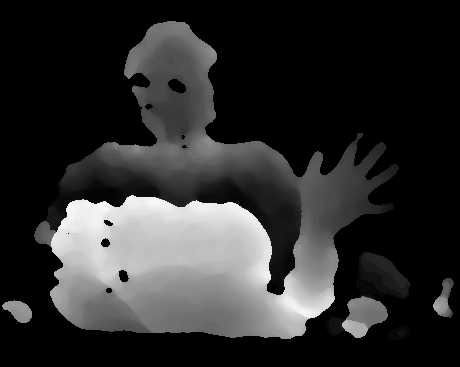
\includegraphics[scale=.25]{./Figures/G3_30.png}\label{fig:G3:3}}
\subfigure[Cuadro número 45 ]{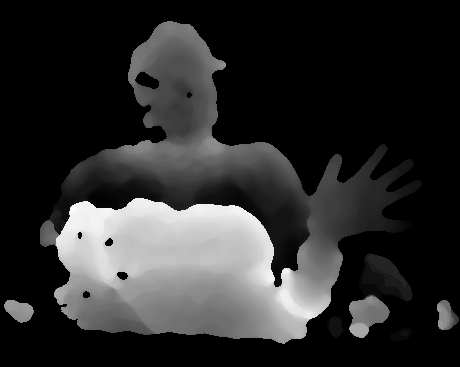
\includegraphics[scale=.25]{./Figures/G3_45.png}\label{fig:G3:4}}
\subfigure[Cuadro final]{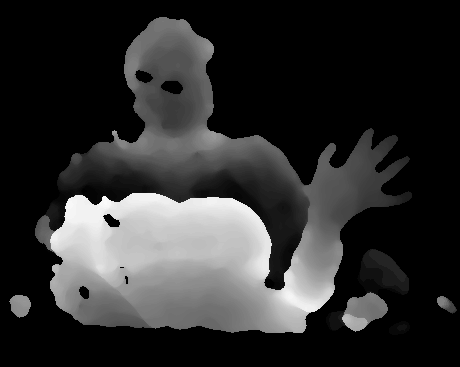
\includegraphics[scale=.25]{./Figures/G3_60.png}\label{fig:G3:5}}
\end{center}
\caption{Secuencia del gesto dinámico de la palma de la mano con los dedos separados, la vista es desde el Kinect frontal.}
\label{fig:G3}
\end{figure}

\begin{figure}[h!]
\begin{center}
\subfigure[Cuadro inicial]{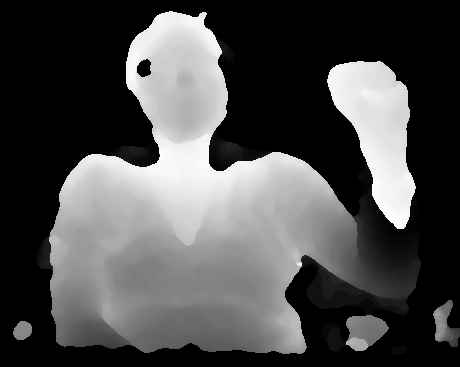
\includegraphics[scale=.25]{./Figures/G4_1.png}\label{fig:G4:1}}  
\subfigure[Cuadro número 15 ]{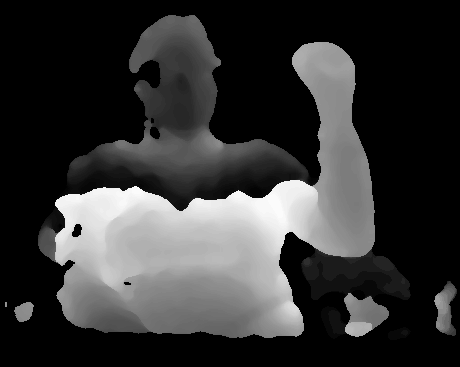
\includegraphics[scale=.25]{./Figures/G4_15.png}\label{fig:G4:2}}
\subfigure[Cuadro número 30 ]{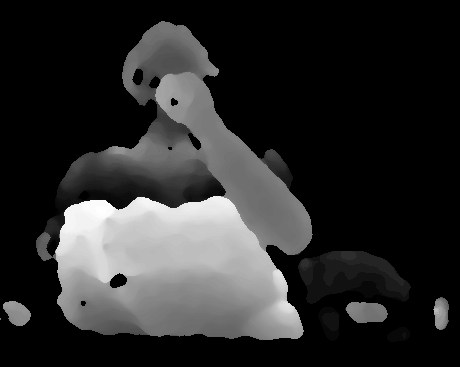
\includegraphics[scale=.25]{./Figures/G4_30.png}\label{fig:G4:3}}
\subfigure[Cuadro número 45 ]{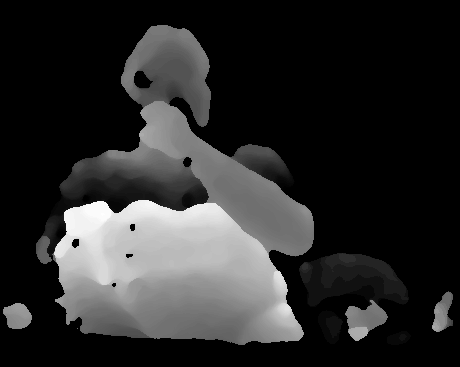
\includegraphics[scale=.25]{./Figures/G4_45.png}\label{fig:G4:4}}
\subfigure[Cuadro final]{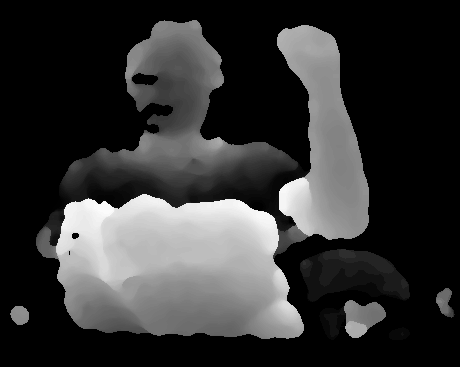
\includegraphics[scale=.25]{./Figures/G4_60.png}\label{fig:G4:5}}
\end{center}
\caption{Secuencia del gesto dinámico del puño, la vista es desde el Kinect frontal.}
\label{fig:G4}
\end{figure}
	
\newpage
%%=====================================================

